\documentclass{article}
\usepackage[a4paper, total={6in, 8in}]{geometry}
\usepackage[utf8]{inputenc}
\frenchspacing

% ------------------------------------------------------------
\usepackage{caption}
\captionsetup{labelformat=empty,labelsep=none}
\usepackage{scalerel,stackengine,amsmath}
\usepackage{mathtools}
\usepackage{dsfont}
\usepackage{multicol}
\usepackage{algorithm2e}
\usepackage{amsfonts}
\usepackage{enumerate}
\usepackage{enumitem}
% ------------------------------------------------------------

% image
\newcommand{\incl}[2]{\includegraphics[width=#1\textwidth]{#2}}
\newcommand{\inclc}[2]{\begin{center}\includegraphics[width=#1\textwidth]{#2}\end{center}}
% description
\newcommand{\thetitle}{}
\newcommand{\thecontents}{}
\newcommand{\thedate}{}
\newcommand{\theauthor}{}
\newcommand{\thedescription}{
	\section*{\thetitle}
	\begin{tabular}{ll}%
	Inhalt:&\thecontents\\%
	Datum:&\thedate\\%
	Author:&\theauthor\\%
	\end{tabular}%
}
% -- math mode stuff
\newcommand{\meq}[1]{\begin{equation*}\begin{aligned}#1\end{aligned}\end{equation*}}
% \newcommand{\NN}{\mathbb{N}}
\newcommand{\NN}{\mathbb{N}}
\newcommand{\ZZ}{\mathbb{Z}}
\newcommand{\QQ}{\mathbb{Q}}
\newcommand{\RR}{\mathbb{R}}
\newcommand{\CC}{\mathbb{C}}
\newcommand{\subt}[1]{\normalfont{(#1)}}
\newcommand{\ifcases}[2]{\begin{equation*}#1\begin{cases}#2\end{cases}\end{equation*}}
\newcommand{\ring}[1]{(#1,+,\cdot)}
\newcommand{\estimates}{\mathrel{\hat{=}}}
\newcommand{\OO}{\mathcal{O}}
\newcommand{\LRA}{\Leftrightarrow}
\newcommand{\LA}{\Leftarrow}
\newcommand{\RA}{\Rightarrow}
\newcommand{\textabove}[2]{\mathrel{\stackrel{\makebox[0pt]{\mbox{\normalfont\tiny #1}}}{#2}}}
\newcommand{\myqed}[1]{\hfill$\Box${\footnotesize#1}}
\newcommand{\neo}[1]{\begin{pmatrix}#1\end{pmatrix}}
\newcommand{\SsS}{\mathcal{S}}
\newcommand{\correct}{\hfill\checkmark}
\newcommand{\ubr}[2]{\underbrace{#1}_{\mathclap{\text{#2}}}}
\newcommand{\obr}[2]{\overbrace{#1}^{\mathclap{\text{#2}}}}
\renewcommand{\star}{^*}
\newcommand{\blank}{\ttt{\textvisiblespace}}
\newcommand\equalhat{\mathrel{\stackon[1.5pt]{=}{\stretchto{%
    \scalerel*[\widthof{=}]{\wedge}{\rule{1ex}{3ex}}}{0.5ex}}}}
\newcommand{\correspondsto}{\equalhat}
\newcommand{\weg}{(weggelassen)}
\newcommand{\chf}{\mathds{1}}
	% -- enumerations
\newcommand{\abc}[1]{\begin{enumerate}[label=\alph*.]#1\end{enumerate}}
\newcommand{\num}[1]{\begin{enumerate}[label=\arabic*.]#1\end{enumerate}}
\newcommand{\bul}[1]{\begin{itemize}#1\end{itemize}}
% -- text mode stuff
% \newcommand{\note}[1]{(\textit{#1})}
\newcommand{\ttt}{\texttt}
\newcommand{\tbf}{\textbf}
\newcommand{\tit}{\textit}
\newcommand{\trt}{\textit}
\newcommand{\tsc}{\textsc}
\newcommand{\tul}{\underline}
\newcommand{\tsub}[1]{\tre{\large#1}}
% -- text input stuff
\newcommand{\ditto}{''}
% <warning_emoji>
\newcommand*{\TakeFourierOrnament}[1]{{%
\fontencoding{U}\fontfamily{futs}\selectfont\char#1}}
\newcommand*{\warning}{\TakeFourierOrnament{66}}
\newcommand{\warn}{{\Large\warning}\ \ }
% </warning_emoji>
% logic stuff
\newcommand{\tttrue}{\ttt{true}}
\newcommand{\fffalse}{\ttt{false}}
% algorithm stuff:
\newcommand{\wwhile}{\textbf{while}}
\newcommand{\ffor}{\textbf{for}}
\newcommand{\ggoto}{\textbf{goto}}
\newcommand{\ddo}{\textbf{do}}
\newcommand{\iif}{\textbf{if}}
\newcommand{\tthen}{\textbf{then}}
\newcommand{\eelse}{\textbf{else}}
\newcommand{\eend}{\textbf{end}}
\newcommand{\hhalt}{\textbf{halt}}
\newcommand{\aand}{\textbf{and}}
\newcommand{\oor}{\textbf{or}}
\newcommand{\ffunction}{\textbf{function}}
\newcommand{\rreturn}{\textbf{return}}
\newcommand{\cccc}{\hphantom{cccc}}
\newcommand{\ccc}{\hphantom{ccc}}
\newcommand{\cc}{\hphantom{cc}}
\renewcommand{\;}{;\\}
\newcommand{\cmt}[1]{\ttt{#1}}
\newcommand{\lims}{\limsup_{n\to\infty}}
\newcommand{\limi}{\liminf_{n\to\infty}}
\newcommand{\true}{\ttt{true}}
\newcommand{\false}{\ttt{false}}


% <local>
\usepackage{hyperref}
\usepackage{url}
\usepackage{tikz}
\usepackage{titlesec}
\usepackage{marvosym}
% --------
\newcommand{\pickl}[1]{\begin{center}\hrulefill\ \texttt{[ \textbf{Pickl #1} ]}\ \hrulefill\end{center}}
\newcommand{\PP}{\mathbb{P}}
\renewcommand{\thesection}{\Roman{section}}
\setcounter{tocdepth}{2}
\renewcommand{\contentsname}{Inhaltsverzeichnis}
% </local>

\begin{document}
\begin{center}
    {\huge{\textsc{\textbf{Stochastik}}}}
\end{center}
Dies ist eine Live-Transkription der Vorlesung Stochastik, gehalten von \tbf{Prof. Dr. Peter Pickl} im \tbf{Sommersemester 2024} an der Uni T\"ubingen.
\\~\\
Dieser Mitschrieb ist fehlerbehaftet und wurde nicht korrekturgelesen. Korrekturhinweise bitte an \href{mailto:thomas.hua@student.uni-tuebingen.de}{\url{thomas.hua@student.uni-tuebingen.de}} bzw. auf GitHub (\href{https://github.com/thomasxhua/stochastik-pickl-ss24-skript/}{\url{https://github.com/thomasxhua/stochastik-pickl-ss24-skript/}}).
\tableofcontents
\newpage

\pickl{15.04.2024}
\trt{In der Stochastik geht es um die Modellierung von Experimenten, deren Ausgang vom Zufall abh\"angt.}
\section{Endliche Wahrscheinlichkeitsr\"aume}
\subsection{Ergebnismenge, Ereignismenge}
\subsubsection{Definition (Ergebnismenge)}
Die Menge $\Omega$, welche die m\"oglichen Ausg\"ange eines Zufallexperiementes beschreibt, dennen wir \trt{Grundmenge} oder \trt{Ergebnismenge}.
\subsubsection{Definition (Ereignismenge)}
Die Potenzmenge $\mathcal{P}(\Omega)$, d.h. die Menge aller Teilmengen $\Omega$, nennen wir \trt{Ereignismenge}.
\subsubsection{Beispiel}
\num{
\item Wir werfen einen W\"urfel.
\bul{
\item $\Omega=\{1,2,\ldots,6\}$,
\item $\mathcal{P}(\Omega)=\{\emptyset,\Omega,\{1\},\ldots,\{1,1\},\ldots\}$,
}
\item Gl\"ucksrad: $\Omega=[0,2\pi[$ beschreibt die m\"oglichen Winkel eines Gl\"uckradspiels. $\mathcal{P}(\Omega)$ ist klar (keine geeignete Ereignismenge, siehe Kapitel 2).
}
\subsection{Wahrscheinlichkeitsma\ss{}}
Das Wahrscheinlichkeitsma\ss{} wird auf der Ereignismenge definiert. Grund: F\"ur \"uberabz\"ahlbare Mengen (Gl\"ucksrad z.B.) haben einzelne Ausg\"ange h\"aufig Wahrscheinlichkeit $0$, obwohl global gesehen existiert ein sinnvolles Wahrscheinlichkeitsma\ss{} (siehe Kapitel 2).
\\~\\
Die Wahrscheinlichkeit quantifiziert die Plausibilit\"at der entsprechenden Ereignisse. Sie gibt die relative H\"aufigkeit an, wie oft ein bestimmtes Ereignis nach sehr h\"aufigen Wiederholen unter identischen Umst\"anden eintritt.
\subsubsection{Definition (Wahrscheinlichkeitsma\ss{})}
Eine Abbildung $\PP\colon\mathcal{P}(\Omega)\to\RR$ nennt man \trt{Wahrscheinlichkeitsma\ss{}} $:\LRA$
\abc{
\item[\tbf{K}a)] $\PP(A)\geq0,\ \forall A\subset\Omega$,
\item[\tbf{K}b)]  $\PP(\Omega)=1$,
\item[\tbf{K}c)]  $\PP(A\cup B)=\PP(A)+\PP(B),\ \forall A,B\subset\Omega,\ A\cap B=\emptyset$.
}
\subsubsection{Bemerkung}
Die Axiome a)-c) nennt man \trt{Axiome von Kolmogorov} (werden in 2 ebenfalls leicht angepasst).
\subsubsection{Satz}
F\"ur jedes Wahrscheinlichkeitsma\ss{} $\PP\colon\mathcal{P}(\Omega)\to\RR$ f\"ur beliebiges $\Omega$ gelten:
\abc{
\item $\PP(A^C)=1-\PP(A),\ \forall A\subset\Omega$.
\item $\PP(A)\leq1$.
\item $\PP(A\cup B)=\PP(A)+\PP(B)-\PP(A\cap B)$.
}
\subsubsection{Beweis}
\weg
\subsubsection{Bemerkung}
\"Uber die Wahrscheinlichkeiten der Elementarereignisse (d.h. der einelementigen Ereignisse), wird das Wahrscheinlichkeitsma\ss{} eindeutig festgelegt.
\\~\\
Betrachte $\PP(A)$ f\"ur $A=\{w_1,w_2,\ldots,w_k\}\subset\Omega$. Durch mehrmaliges Anwenden von \tbf{K}c) erh\"alt man
\meq{\PP(A)=\sum_{i=1}^{k}\PP(\{w_k\}).}
\subsubsection{Definition (Wahrscheinlichkeitsraum)}
Das Paar $(\Omega,\PP)$ nennt man auch \trt{Wahrscheinlichkeitsraum} (auch $(\Omega,\mathcal{P}(\Omega),\PP)$).


\pickl{18.04.2024}
\subsubsection{Bemerkung}
Wie findet man nun das richtige Wahrscheinlichkeitsma\ss{}, d.h. jenes, welches zu meinem Experiment passt?
\num{
\item Ausprobieren (siehe unten, ``Statistik'').
\item Analyse der physikalischen Eigenschaften. Praktikabel, falls Symmetrie in den relevanten physikalischen Eigenschaften herrscht:
}
\subsubsection{Laplace-Annahme (Indifferenzprinzip)}
Falls es keinen Grund zur Annahme gibt, dass die verschiedenen Ausg\"ange des Experiments im Wesentlichen zu unterscheiden sind, nehmen wir an, dass die Wahrscheinlichkeiten aller Elementarerignisse gleich sind.
\subsubsection{Folgerung}
Sei $\Omega$ ein Ergebnisraum. Unter der Laplace-Annahme gilt:
\[
\mathbb{P}(A)=\frac{|A|}{|\Omega|}
\]
\subsubsection{Beweis}
\[
1\textabove{\tbf{K}}{=}\mathbb{P}(\Omega)=\mathbb{P}(\bigcup_{\omega\in\Omega}\{\omega\})\textabove{\tbf{K}}{=}\sum_{\omega\in\Omega}\mathbb{P}(\{\omega\})\textabove{\tbf{L}}{=}|\Omega|\cdot\mathbb{P}(\{\omega\})
\]
$\Rightarrow\forall\omega\in\Omega$ gilt:
\[
\mathbb{P}(\{w\})=\frac{1}{|\Omega|}.
\]
Au\ss{}erdem:
\[
\mathbb{P}(A)=\mathbb{P}(\bigcup_{\omega\in A}\{\omega\})\textabove{\tbf{K}}{=}\sum_{\omega\in A}\mathbb{P}(\{\omega\})=|A|\cdot\frac{1}{|\Omega|}.
\]
\subsubsection{Beispiel}
\num{
\item Werfen eines ungezinkten W\"urfels:
\[
\mathbb{P}(\{2,4,6\})=\frac{3}{6}=\frac{1}{2}.
\]
\item Gesamte Augenzahl bei zweimaligen Werfen des W\"urfels
\[
\Omega=\{2,\ldots,12\},
\]
Laplace-Annahme gilt nicht. Die Elemente sind wesentlich verschieden, z.B. $2$ hat nur Option $(1,1)$, $7$ hat die Optionen $\{(1,6),\ldots\}$.
\item Ziegenproblem: Wir befinden uns in einer Gameshow, d\"urfen zwischen drei Toren w\"ahlen. Hinter einemal Tor ist ein Gewinn, hinter zweien eine Niete. Der Moderator \"offnet eines der nicht-gew\"ahlten Tore. Hinter diesen ist eine Niete. Er bietet daraufhin an, das Tor zu wechseln. Ist der Wechsel sinnvoll?
\bul{
\item Problem 1: Spielregeln m\"ussen erg\"anzt werden. Wie handelt der Moderator? Wir gehen davon aus, dass er oder sie in jedem Fall ein nicht-gew\"ahltes Tor mit Niete \"offnet.
\item Problem 2: Man ist geneigt, von einer Laplace-Situation auszugehen. Dies ist falsch, da die Tore durch die Wahl und die Reaktion des Moderators zu unterscheiden sind.
}
}
\begin{center}
\begin{minipage}{0.45\textwidth}
\centering
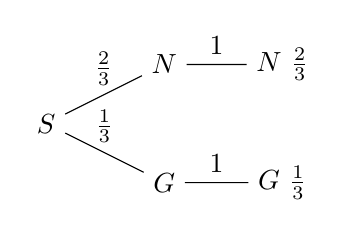
\begin{tikzpicture}[grow=right]
    \node {$S$}
        child
        {
            node {$G$}
            child
            {
                node {$G\ \frac{1}{3}$}
                edge from parent node[above] {$1$}
            }
            edge from parent node[above] {$\frac{1}{3}$}
        }
        child
        {
            node {$N$}
            child
            {
                node {$N\ \frac{2}{3}$}
                edge from parent node[above] {$1$}
            }
            edge from parent node[above] {$\frac{2}{3}$}
        };
\end{tikzpicture}\\
Ohne Wechseln
\end{minipage}
\begin{minipage}{0.45\textwidth}
\centering
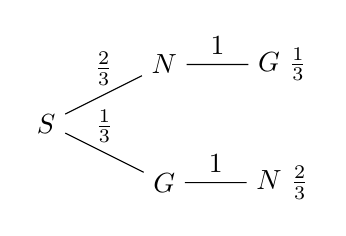
\begin{tikzpicture}[grow=right]
    \node {$S$}
        child
        {
            node {$G$}
            child
            {
                node {$N\ \frac{2}{3}$}
                edge from parent node[above] {$1$}
            }
            edge from parent node[above] {$\frac{1}{3}$}
        }
        child
        {
            node {$N$}
            child
            {
                node {$G\ \frac{1}{3}$}
                edge from parent node[above] {$1$}
            }
            edge from parent node[above] {$\frac{2}{3}$}
        };
\end{tikzpicture}\\
Mit Wechseln
\end{minipage}
\end{center}
mit Start ($S$), Gewinn ($G$) und Niete ($N$).
\subsection{Kombinatorik}
Wie bestimmt man in einer Laplace-Situation $|A|$ und $|\Omega|$?
\subsubsection{Beispiele}
\abc{
\item Sei $\Omega=A\times B$, so ist $|\Omega|=|A|\cdot|B|$ M\"unzwurf, dann W\"urfel:
\[
A=\{\text{K},\text{Z}\},\ B=\{1,\ldots,6\}.
\]
\item Urne mit $N$ durchnummerierten Kugeln. Wir ziehen davon nacheinander ohne Zur\"ucklegen $k$ Kugeln (Reihenfolge wird ber\"ucksichtigt):
\[
|\Omega|=N(N-1)\ldots(N-k+1)=\frac{N!}{(N-k)!}.
\]
\item Zahlenlotto ``6 aus 49'', wie b) ohne R\"ucksicht auf Reihenfolge:
\[
|\Omega|=\frac{N!}{(N-k)!}\cdot\frac{1}{k!}.
\]
\item Anzahl der Anagramme von \ttt{MISSISSIPPI}.
\[
|\Omega|=\frac{11!}{\ubr{4!}{\ttt{I}}\ubr{4!}{\ttt{S}}\ubr{2!}{\ttt{P}}}.
\]
}
\newpage
\section{Allgemeine Wahrscheinlichkeitsr\"aume}
\setcounter{subsection}{-1}
\subsection{Anpassung des 3. Axioms von Kolmogorov}
Wir werden das 3. Axiom von Kolmogorov anpassen:
\[
\mathbb{P}(\bigcup_{j=1}^\infty A_j)=\sum_{j=1}^\infty\mathbb{P}(A_j),\ \text{falls}\ A_j\cap A_k=\emptyset,\ \forall j\neq k.
\]
Schwieriger ist die anpassung des Definitionsbereiches von $\mathbb{P}$. Warum ist das n\"otig? Betrachte das Beispiel ``Gl\"ucksrad''. 

\pickl{22.04.2024}
\subsubsection{Lemma}
Es gibt kein translationsinvariantes Wahrscheinlichkeitsma\ss{} auf $\PP([0,2\pi[)$.
\subsubsection{Beweis}
WA: Es gibt ein solches $\PP$.
\\~\\
Wir zerlegen nun $[0,2\pi[$ in \"uberabz\"ahlbar viele abz\"ahlbare Teilmengen:
\meq{a~b:\LRA a-b\in\QQ.}
Dies definiert \"Aquivalenzklassen, diese dienen zur Zerlegung von $[0,2\pi[$:
\bul{
\item $\{0,\frac{1}{2},\frac{1}{3},1,\ldots\}$,
\item $\{\sqrt{2},\sqrt{2}+\frac{1}{2},\ldots\}$,
\item $\{\pi,\pi+\frac{1}{2},\ldots\}$,
\item \ldots
}
Wir w\"ahlen aus jeder \"Aquivalenzklasse einen Representanten $\leftarrow\{0,\sqrt{2},\pi,\ldots\}$. $R$ ist nat\"urlich \"uberabz\"ahlbar. F\"ur jedes $q\in[0,2\pi[\cap\QQ$ definieren wir
\meq{R_q:=\{r+q,\ r\in R\}=R+q.}
Nach Annahme der Translationsinvarianz ist
\meq{\PP(R_q)=\PP(R),\ \forall q\in[0,2\pi[\cap\QQ.}
Es gilt:
\meq{{}[0,2\pi[\ \subseteq\ \bigcup_{\mathclap{q\in]-2\pi,2\pi[\cap\QQ}}\ R_q\subset\ ]-2\pi,4\pi[.}
$\RA$ da $\PP([0,2\pi[)=1$, gilt, dass
\meq{
    &\PP(\bigcup_{\mathclap{q\in]-2\pi,2\pi[\cap\QQ}}R_q)\geq1.\\
    \RA\ &\sum_{\mathclap{j\in]-2\pi,2\pi[}}\PP(R)\geq1\\
    \RA\ &\PP(R)\neq0,
}
aber falls der Inhalt $\PP(R)>0$, folgt, dass das Intervall $]-2\pi,4\pi[$ unendlichen Inhalt hat. Dieses \"uberdeckt jedoch $[0,2\pi[$ dreimal. $\lightning$
\subsection{Ereignisraum}
Wir schr\"anken den Definitionsbereich von $\PP$ ein, um solch problematische Mengen zu umgehen. 
\subsubsection{$\sigma$-Algebra}
Sei $\Omega$ eine Menge. Eine $\sigma$-Algebra bzgl. $\Omega$ ist eine Teilmenge von $\mathcal{P}(\Omega)$ mit:
\abc{
\item $\Omega\in\mathcal{A}$,
\item $A\in\mathcal{A}\RA A^C\in\mathcal{A}$,
\item Sei $(A_n)_{n\in\NN}\subset\mathcal{A}\RA\bigcup_{n=1}^\infty A_n\in\mathcal{A}$.
}
\subsubsection{Beispiele}
\abc{
\item $\mathcal{P}(\Omega)$, sowie $\{\emptyset,\Omega\}$ ist jeweils $\sigma$-Algebra.
\item
    \bul{
    \item $\Omega=\{1,2,3,4\}$.
    \item $\mathcal{A}=\{\emptyset,\Omega,\{1,2\},\{3\},\{4\},\{3,4\},\{1,2,4\},\{1,2,3\}\}$.
    }
}
\subsubsection{Satz}
Sei $\mathcal{A}$ eine $\sigma$-Algebra bzgl. $\Omega$. Dann gilt:
\abc{
\item $\emptyset\in\mathcal{A}$,
\item abz\"ahlbare Schritte von Ereignissen sind in $\mathcal{A}$,
\item $A,B\in\mathcal{A}\RA A\setminus B\in\mathcal{A}$.
}
\subsubsection{Beweis}
\abc{
\item $\emptyset=\Omega^C\in\mathcal{A}$,
\item $\bigcap_{n=1}^\infty A_n=\left[\bigcup_{n=1}^\infty A^C_n\right]^C\in\mathcal{A}$,
\item $A\setminus B=A\cap B^C$.
}
\subsubsection{Satz}
Sei $\Omega$ eine Menge. Der Schnitt beliebiger $\sigma$-Algebren ergibt wieder eine $\sigma$-Algebra.
\subsubsection{Beweis}
Seien $\mathcal{A}_i$ f\"ur $i\in\mathcal{I}$ $\sigma$-Algebren (bzgl. $\Omega$). Z.z. $\mathcal{A}:=\bigcap_{i\in\mathcal{I}}\mathcal{A}_i$ ist $\sigma$-Algebra.
\abc{
\item $\Omega\in\mathcal{A}_i,\ \forall i\in\mathcal{I}\RA\Omega\in\mathcal{A}.$
\item Sei $E\in\mathcal{A}\RA E\in\mathcal{A}_i,\ \forall i\in\mathcal{I}\RA E^C\in\mathcal{A}_i,\ \forall i\in\mathcal{I}$.
\item Seien $(E_n)_{n\in\NN}\subset\mathcal{A}$ ($E_n\in\mathcal{A}\ \forall n\in\NN$):
\meq{
    \RA\ &E_n\in A_i,\ \forall n\in\NN, \forall i\in\mathcal{I}\\
    \RA\ &\bigcup_{n=1}^\infty E_n\in\mathcal{A}_i,\ \forall i\in\mathcal{I}\ \text{(da $\mathcal{A}_i$ $\sigma$-Algebra)}\\
    \RA\ &\bigcup_{n=1}^\infty E_n\in\mathcal{A}.
}
}
\subsubsection{Bemerkung}
Vereinigungen von $\sigma$-Algebren ergeben \trt{nicht} notwendigerweise eine $\sigma$-Algebra.
\subsubsection{Beispiel}
$\Omega=\{1,2,3\}$.
\bul{
\item $\mathcal{A}_1=\{\Omega,\emptyset,\{1,2\},\{3\}\}$,
\item $\mathcal{A}_2=\{\Omega,\emptyset,\{1,3\},\{2\}\}$,
\item $\mathcal{A}_1\cup\mathcal{A}_2=\{\Omega,\emptyset,\{1,2\},\{1,3\},\{2\},\{3\}\}\not\ni\{2\}\cup\{3\}.$
}
\subsubsection{Definition (Erzeugte $\sigma$-Algebra)}
Sei $\Omega$ eine Menge, $\mathcal{E}\subset\mathcal{P}(\Omega)$. Die $\sigma$-Algebra $\sigma(\mathcal{E})$ definiert durch
\meq{\sigma(\mathcal{E}):=\bigcap_{\mathclap{\mathcal{A}\text{ ist $\sigma$-Alg},\ \mathcal{E}\subset\mathcal{A}}}\mathcal{A}}
nennen wir die \trt{von $\mathcal{E}$ erzeugte $\sigma$-Algebra}.
\subsubsection{Bemerkung}
$\sigma(\mathcal{E})$ ist f\"ur nichtleere $\Omega$ immer wohldefiniert und wegen Satz $\sigma$-Algebra.
\subsubsection{Korollar}
$\sigma(\mathcal{E})$ ist die kleinste $\sigma$-Algebra, die $\mathcal{E}$ enth\"alt, d.h.
\abc{
\item $\mathcal{E}\in\sigma(\mathcal{E})$,
\item $\forall\widetilde{\mathcal{A}}$ $\sigma$-Algebra it $\mathcal{E}\subset\widetilde{\mathcal{A}}$, gilt $\sigma(\mathcal{E})\subset\widetilde{\mathcal{A}}$.
}
\subsubsection{Beweis}
\abc{
\item $\mathcal{E}$ ist in allen $\sigma$-Algebren enthalten, \"uber die der Schnitt gebildet wird.
\item $\widetilde{\mathcal{A}}$ ist ein Kandidat f\"ur $\mathcal{A}$ in der Definition. Es wird also auch \"uber $\widetilde{\mathcal{A}}$ der Schnitt gebildet $\RA\widetilde{A}\supset\sigma(\mathcal{E})$.
}
\subsubsection{Beispiel}
$\Omega=\{1,2,3\},\mathcal{E}=\{\{1,2\}\}$. $\mathcal{P}(\Omega)$ ist $\sigma$-Algebra, enth\"alt $\mathcal{E}$ $\mathcal{A}_1$ vom Beispiel oben ebenso. Weitere Kandidaten:
\meq{\mathcal{B}=\{\Omega,\emptyset,\{1,2\},\{3\},\{1\},\{2\},\ldots\}.}


\pickl{25.04.2024}
\subsubsection{Defintion (Borel-$\sigma$-Algebra)}
Sei $\Omega=\mathbb{R}$. Die von den offenen Teilmengen von $\mathbb{R}$ erzeugte $\sigma$-Algebra hei\ss{}t \trt{Borel-$\sigma$-Algebra}. (alternative Definiton sp\"ater)
\subsection{Wahrscheinlichkeitsma\ss{}}
\subsubsection{Definition (Wahrscheinlichkeitsma\ss{})}
Sei $\Omega$ eine Menge, $\mathcal{A}$ $\sigma$-Algebra. Eine Abbildung $\mathbb{P}\colon\mathcal{A}\to\mathbb{R}$ hei\ss{}t \trt{Wahrscheinlichkeitsma\ss{}} $:\LRA$
\abc{
\item $\mathbb{P}(\Omega)=1$,
\item $\mathbb{P}(A)\geq0,\ \forall A\in\mathcal{A}$,
\item $\mathbb{P}(\bigcup_{n=1}^\infty A_n)=\sum_{n=1}^\infty\mathbb{P}(A_n)$, falls $A_n\in\mathcal{A},\ A_n\cap A_m=\emptyset\ \forall n\neq m$.
}
\subsubsection{Bemerkung}
Satz vom Gegenereignis, $\mathbb{P}(\emptyset)=0$ und $\mathbb{P}(A\cup B)=\mathbb{P}(A)+\mathbb{P}(B)-\mathbb{P}(A\cap B)$ gilt weiterhin.
\subsubsection{Definition und Satz (Bedingte Wahrscheinlichkeit)}
Sei $(\Omega,\mathcal{A},\mathbb{P})$ ein Wahrscheinlichkeitsraum, d.h. $\Omega$ Menge, $\mathcal{A}$ zugeh\"orige $\sigma$-Algebra, $\mathbb{P}\colon\AA\to\mathbb{R}$ Wahrscheinlichkeitsma\ss{}.
\\~\\
Sei $A\in\mathcal{A}$ mit $\mathbb{P}(A)\neq0$. Dann ist das auf $A$ \trt{bedingte Wahrscheinlichkeitsma\ss{}} definiert durch
\[
\mathbb{P}_A(B)=\frac{\mathbb{P}(A\cap B)}{\mathbb{P}(A)}.
\]
\subsubsection{Beweis}
(dass dies ein Wahrscheinlichkeitsma\ss{} ist):
\abc{
\item $\mathbb{P}_A(\Omega)=\frac{\mathbb{P}(A\cap\Omega)}{\mathbb{P}(A)}=\frac{\mathbb{P}(A)}{\mathbb{P}(A)}=1.$
\item Z\"ahler $\geq0$, Nenner $>0$ $\RA$ Behauptung.
\item 
\begin{align*}
    \mathbb{P}_A(\bigcup_{n=1}^\infty A_n)&=\frac{\mathbb{P}(A\ \cap\ \bigcup_{n=1}^\infty A_n)}{\mathbb{P}(A)}\ (A_n\cap A_m=\emptyset,\ n\neq m)\\
    &=\frac{\mathbb{P}(\bigcup_{n=1}^\infty\obr{(A_n\cap A)}{paarweise disjunkt})}{\mathbb{P}(A)}\\
    &=\frac{\sum_{n=1}^\infty\mathbb{P}(A_n\cap A)}{\mathbb{P}(A)}\\
    &=\sum_{n=1}^\infty\mathbb{P}_A(A_n).
\end{align*}
}
\subsubsection{Definition (Unabh\"angigkeit)}
Zwei Ereignisse $A,B$ hei\ss{}en (stochastisch) \trt{unabh\"angig} $:\LRA$
\[
\mathbb{P}(A\cap B)=\mathbb{P}(A)\cdot\mathbb{P}(B).
\]
\subsubsection{Bemerkung}
$A$ unabh\"angig von $B$ $\RA$ $\mathbb{P}_A(B)=\mathbb{P}(B)$ (falls $\mathbb{P}(A)\neq0$).
\subsubsection{Beispiel}
$\Omega=\{1,\ldots,6\}$.
\abc{
\item $A=\{3,4,5,6\},\ B=\{2,4,6\}$ sind unabh\"angig.
\item $\widetilde{A}=\{4,5,6\}$ und $B$ wie oben sind nicht unabh\"angig.
}
\subsubsection{Definition (Limes von Ereignissen)}
Seien $(A_n)_{n\in\mathbb{N}}\subset\mathcal{A}$, $(B_n)_{n\in\mathbb{N}}\subset\mathcal{A}$.
Wir nehmen an:
\bul{
\item $A_n\subset A_{n+1},\ \forall n\in\mathbb{N}$,
\item $B_n\supset B_{n+1},\ \forall n\in\mathbb{N}$.
}
Dann ist
\begin{align*}
    \lim_{n\to\infty}A_n&\ :=\bigcup_{n=1}^\infty A_n,\\
    \lim_{n\to\infty}B_n&\ :=\bigcap_{n=1}^\infty B_n.
\end{align*}
\subsubsection{Korrolar}
$\lim_{n\to\infty}A_n$ und $\lim_{n\to\infty}B_n$ sind Ereignisse, falls $A_n$, $B_n$ Ereignisse sind.
\subsubsection{Beweis}
Definition der $\sigma$-Algebra, bzw. Satz gleich darunter.
\subsubsection{Definition ($\limsup$, $\liminf$)}
Sei $(A_n)_{n\in\mathbb{N}}\subset\mathcal{A}$ Dann ist
\begin{align*}
\limsup_{n\to\infty}A_n&\ :=\bigcap_{k=1}^\infty\bigcup_{n=k}^\infty A_n,\\
\liminf_{n\to\infty}A_n&\ :=\bigcup_{k=1}^\infty\bigcap_{n=k}^\infty A_n.
\end{align*}
\subsubsection{Korollar}
Auch $\limsup$ und $\liminf$ sind Ereignisse (falls $A_n\in\mathcal{A}\ \forall n\in\mathbb{N}$).
\subsubsection{Satz ($\sigma$-Stetigkeit des Wahrscheinlichkeitsma\ss{}es)}
Sei $(A_n)_{n\in\mathbb{N}},(B_n)_{n\in\mathbb{N}}\subset\mathcal{A}$ eine abfallende bzw. ansteigende Folge von Ereignissen ($A_n\subset A_{n+1},\ B_n\supset B_{n+1},\ \forall n$). Dann ist
\abc{
\item $\lim_{n\to\infty}\mathbb{P}(A_n)=\mathbb{P}(\lim_{n\to\infty}A_n)$,
\item $\lim_{n\to\infty}\mathbb{P}(B_n)=\mathbb{P}(\lim_{n\to\infty}B_n)$.
}
\subsubsection{Beweis}
Definiere $C_1:=A_1$. $C_2:=A_1\setminus A_1$, \ldots, $C_n=A_n\setminus A_{n-1}$. Es gilt:
\abc{
\item $\lim_{n\to\infty}A_n=\bigcup_{n=1}^\infty A_n=\bigcup_{n=1}^\infty C_n$.
\item $C_n\cap C_m=\emptyset,\ \forall n\neq m$,
\item $A_n=\bigcup_{k=1}^{n}C_k$.
}
\abc{
\item
\begin{align*}
    \RA\mathbb{P}(\lim_{\mathclap{n\to\infty}}A_n)&\ \textabove{a)}{=}\mathbb{P}(\bigcup_{n=1}^\infty C_n)
    \\&\ \textabove{\tbf{K}c)}{=}\sum_{n=1}^\infty\mathbb{P}(C_n)
    \\&\ =\lim_{n\to\infty}\sigma_{k=1}^{n}\mathbb{P}(C_k)
    \\&\ \textabove{\tbf{K}c)}{=}\lim_{n\to\infty}\mathbb{P}(\bigcup_{k=1}^nC_k)
    \\&\ \textabove{c)}{=}\mathbb{P}(A_n).
\end{align*}
\myqed{}
\item
\begin{align*}
    \mathbb{P}(\lim_{\mathclap{n\to\infty}}B_n)&\ =1-\mathbb{P}(\lim_{\mathclap{n\to\infty}}B_n^C)
    \\&\ \textabove{Fall a)}{=}\ 1-\lim_{n\to\infty}\mathbb{P}(B_n^C)
    \\&\ =\lim_{n\to\infty}\mathbb{P}(B_n).
\end{align*}
}

\pickl{29.04.2024}
\subsection{Borelsche $\sigma$-Algebra}
\subsubsection{Erinnerung}
$\mathcal{B}^\RR$ ist die $\sigma$-Algebra erzeugt aus allen offenen Teilmengen von $\RR$.
\subsubsection{Bemerkung}
Diese Definition l\"asst sich auf Grundmengen verallgemeinern, in denen es ein ``Konzept'' von offenen Teilmengen gibt (topologische R\"aume, z.B. metrische R\"aume). Wir werden alternative Definitionen von $\mathcal{B}$ betrachten.
\subsubsection{Korollar}
\abc{
\item Sei $\mathcal{E}\subset\mathcal{P}(\Omega),$ $\mathcal{A}\subset\mathcal{P}(\Omega)$ $\sigma$-Algebra. $\mathcal{E}\subset\mathcal{A}\RA\sigma(\mathcal{E})\subset\mathcal{A}$.
\item Seien $\mathcal{E},\mathcal{F}\subset\mathcal{P}(\Omega)$. Falls $\mathcal{E}\subset\sigma(\mathcal{F})$ und $\mathcal{F}\subset\sigma(\mathcal{E})\RA\sigma(\mathcal{E})=\sigma(\mathcal{F})$.
}
\subsubsection{Beweis}
\abc{
\item \[\sigma(\mathcal{E})=\bigcap_{\mathclap{\mathcal{B}\ \sigma\text{-Algebra},\ \mathcal{E}\subset\mathcal{B}}}\mathcal{B}\]
$\leadsto$ $\mathcal{A}$ ist einer der Kandidaten, \"uber die geschnitten wird.
\item
\meq{
\mathcal{E}\subset\sigma(\mathcal{F})&\ \textabove{a)}{\RA}\sigma(\mathcal{E})\subset\sigma(\mathcal{F}),\\
\mathcal{F}\subset\sigma(\mathcal{E})&\ \textabove{a)}{\RA}\sigma(\mathcal{F})\subset\sigma(\mathcal{E}).
}
}
\subsubsection{Satz}
Die Borelsche $\sigma$-Algebra $\mathcal{B}^\RR$ ist die aus den offenen Intervallen erzeugte $\sigma$-Algebra.
\subsubsection{Beweis}
Z.z.: Jede offene Teilmenge $\RR$ liegt in der aus den offenen Intervallen erzeugten $\sigma$-Algebra.
\\~\\
Sei $A\subset\RR$ offen. F\"ur jedes $q\in\QQ\cap A$ sei
\[r_q=\sup\{\varepsilon\in\RR\colon\ ]q-\varepsilon,\ q+\varepsilon[\ \subset A\}.\]
Das Intervall $]q-r_q,\ q+r_q[$ ist $\subset A$ $(*)$. (WA: $]q-r_q,\ q+r_q[\ \not\subset A$ $\RA$ $\exists x\in\ ]q-r_q,\ q+r_q[$ mit $x\notin A$. W\"ahle $\varepsilon=\frac{r_q+|q-x|}{2}$ $\RA$ $x\in\ ]q-r_q,\ q+r_q[$, aber $\varepsilon<r_q$ $\lightning$.)
\\~\\
Betrachte $B=\bigcup_{q\in\QQ\cap A}\ ]q-r_q,\ q+r_q[$. Z.z. $A=B$ (da $B$ abz\"ahlbare Vereinigung offener Intervalle).
\bul{
\item $B\subset A$, da all die Teilintervalle $]q-r_q,\ q+r_q[\ \subset A$ $(*)$.
\item $A\subset B$. Sei $y\in A$. Z.z. $y\in B$. Wegen Offenheit von $A$ $\exists\delta_y$, sodass $]y-\delta_y,\ y+\delta_y[\ \subset A$. W\"ahle $q_y\in\QQ\cap\ ]y-\frac{\delta_y}{2},y+\frac{\delta_y}{2}[$. $r_{q_y}\geq\frac{\delta_y}{2}$ $\RA$ $y\in\ ]q_y-r_{q_y},\ q_y+r_{q_y}[$.
}
\subsubsection{Satz}
Die Borel-$\sigma$-Algebra ist genau die $\sigma$-Algebra erzeugt aus den Intervallen $]-\infty,\ a]$ mit $a\in\RR$.
\subsubsection{Beweis}
$\mathcal{E}:=$ Menge der offenen Intervalle, $\mathcal{F}:=\{]-\infty,\ a],\ a\in\RR\}$.
\abc{
\item Z.z. $\mathcal{E}\subset\sigma(\mathcal{F})$.
\\~\\
Sei $a<b\in\RR\cup\{\pm\infty\}$. Z.z. $]a,b[\ \in\sigma(\mathcal{F})$.
\bul{
\item 1. Schritt: ``$a=-\infty$''.
\[]-\infty,\ b[\ =\ \ubr{\bigcup_{n\in\NN}\ubr{\left]-\infty,\ b-\frac{1}{n}\right]}{$\in\mathcal{F}$}}{$\in\sigma(\mathcal{F})$}.\]
$\forall x\in\ ]-\infty,\ b[$, d.h. $\forall x<b\ \exists n\in\NN$, sodass $x<b-\frac{1}{n}\RA x\in\bigcup_{n\in\NN}\ \left]-\infty,\ b-\frac{1}{n}\right]$.
$\RA\ ]-\infty,\ b[\ \subset\ \bigcup_{n\in\NN}\left]-\infty,\ b-\frac{1}{n}\right]$. $\forall n\in\NN$ ist $\left]-\infty,b-\frac{1}{n}\right]\ \subset\ ]-\infty,b[$ $\RA``\supset''$.
\item 2. Schritt:
\[a\in\RR\colon\ ]a,b[\ =\ \ubr{]-\infty,b[}{$\in\sigma(\mathcal{F})$ (1. Schritt)}\ \setminus\ \obr{]-\infty,a]}{$\in\mathcal{F}\subset\sigma(\mathcal{F})$}\]
nach Satz ist letzteres in $\sigma(\mathcal{F})$.
}
\item Z.z. $\forall a\in\RR$ ist $]-\infty,\ a]\ \in\sigma(\mathcal{E})$.
\[]-\infty,a]\ =\ (]a,\ +\infty[)^C=(\bigcup_{n\in\NN}\ ]a,\ n[)^C.\]
}
\subsubsection{Satz}
$\mathcal{B}^\RR$ ist die $\sigma$-Algebra erzeugt aus $\{]-\infty,a]\ \text{mit}\ a\in\QQ\}$.
\subsubsection{Beweis}
Sei $\mathcal{G}=\{]-\infty,a]\colon a\in\QQ\}$. Offensichtlich ist $\mathcal{G}\subset\mathcal{F}$.
\[\mathcal{G}\subset\mathcal{F}\subset\sigma(\mathcal{F}).\]
Z.z. $\mathcal{F}\subset\sigma(\mathcal{G})$. Sei $]-\infty,a]\ a\in\RR$.
\[]-\infty,a]\ =\ \ubr{\bigcap_{\mathclap{q\in\QQ,\ q\geq a}}\ ]-\infty,\ q]}{$\in\sigma(\mathcal{G})$}.\]
$]-\infty,a]\ \subset\ ]-\infty,q]$, $\forall q\geq a$ $\RA$ $]-\infty,a]\subset\bigcup_{q\in\QQ,\ q\geq a}\ ]-\infty,q]$ ($\RA$ ``$\subset$'').
\\~\\
``$\supset$'': Dazu ``$\subset$'' f\"ur die Komplete. Sei $x\notin]-\infty,\ a]$ $\RA$ $x>a$. W\"ahle $q\in\ ]a,x[\ \cap\QQ\RA x\notin\ ]-\infty,\ q]\ \RA x\notin\bigcup_{q\in\QQ,\ q\geq a}\ ]-\infty,q]$.

\pickl{02.05.2024}
\subsection{Eindeutigkeitssatz}
Ziel ist es zu zeigen, dass unter gewissen Bedingungen das Wahrscheinlichkeitsma\ss{} eindeutig festgelegt ist, falls es auf einem Erzeuger gegeben ist.
\\~\\
Wir benutzen das ``Prinzip der guten Mengen''.
\subsubsection{Satz (Prinzip der guten Mengen)}
Falls eine Eingenschaft f\"ur $\mathcal{E}\subset\mathcal{P}(\Omega)$ gilt und die Menge, auf der die Eigenschaft gilt eine $\sigma$-Algebra ist, so gilt die Eigenschaft auf ganz $\sigma(\mathcal{E})$.
\subsubsection{Beweis}
Sei $\mathcal{A}$ die Menge, f\"ur die die Eigenschaft gilt. Da $\mathcal{E}\subset\mathcal{A}$, $\mathcal{A}$ ist $\sigma$-Algebra nach Voraussetzung,
\[\sigma(\mathcal{E})=\bigcup_{\mathclap{\mathcal{B}\ \text{ist $\sigma$-Algebra},\ \mathcal{E}\subset\mathcal{B}}}\mathcal{B}.\]
$\mathcal{A}$ ist eines der Kandidaten f\"ur $\mathcal{B}$ $\Rightarrow$ $\sigma(\mathcal{E})\subset\mathcal{A}$.
\subsubsection{Beweisstrategie f\"ur den Eindeutigkeitssatz}
Seien $\mathbb{P},\mathbb{Q}\colon\sigma(\mathcal{E})\to\mathbb{R}$ Wahrscheinlichkeitsma\ss{}e. Wir m\"ochten zeigen, dass unter gewissen Bedingungen die Menge $\mathcal{G}$ definiert durch
\[A\in\mathcal{G}\Leftrightarrow\mathbb{P}(A)=\mathbb{Q}(A)\]
eine $\sigma$-Algebra ist.
\\~\\
Nach dem Prinzip der guten Mengen ist dann
\[\mathbb{P}(A)=\mathbb{Q}(A),\ \forall A\in\sigma(\mathcal{E}).\]
Wir beweisen dies in zwei Schritten:
\num{
\item Die Menge $\mathcal{G}$ ist ein Dynkin-System.
\item Unter gewissen Bedingungen ist jedes Dynkin-System eine $\sigma$-Algebra.
}
\subsubsection{Definition (Dynkin-System)}
Eine Teilmenge $\mathcal{D}$ hei\ss{}t \trt{Dynkin-System} $:\Leftrightarrow$
\abc{
\item $\Omega\in\mathcal{D}$,
\item $A\in\mathcal{D}\Rightarrow A^C\in\mathcal{D}$,
\item $(A_n)_{n\in\mathbb{N}}\subset\mathcal{D}$, $A_n$ paarweise disjunkt $\Rightarrow\bigcup_{n\in\mathbb{N}}A_n\in\mathcal{D}$.
}
\subsubsection{Satz}
Seien $\mathbb{P},\mathbb{Q}$ Wahrscheinlichkeitsma\ss{}e auf $\mathcal{A}$. $\mathcal{G}:=\{A\subset\mathcal{A}\colon\mathbb{P}(A)=\mathbb{Q}(A)\}$ ist ein Dynkin-System.
\subsubsection{Beweis}
\abc{
\item $\mathbb{P}(\Omega)=1=\mathbb{Q}(\Omega)\Rightarrow\Omega\in\mathcal{G}$.
\item Sei $A\in\mathcal{G}$, d.h. $\mathbb{P}(A)=\mathbb{Q}(A)\Rightarrow\mathbb{P}(A^C)=1-\mathbb{P}(A)=1-\mathbb{Q}(A)=\mathbb{Q}(A^C)$, d.h. $A^C\in\mathcal{G}$.
\item Sei $(A_n)_{n\in\mathbb{N}}\subset\mathcal{G}$ paarweise disjunkt, d.h. $\mathbb{P}(A_n)=\mathbb{Q}(A_n),\ \forall n\in\mathbb{N}$
\[\Rightarrow\mathbb{P}(\bigcup_{n\in\mathbb{N}}A_n)\textabove{\tbf{K}c)}{=}\Sigma_{n\in\mathbb{N}}\mathbb{P}(A_n)\textabove{$\overleftarrow{\text{\tbf{K}c)}}$}{=}\mathbb{Q}(\bigcup_{n\in\mathbb{N}}A_n).\]
}
\subsubsection{Definition (Schnittstabilit\"at)}
Eine Menge $\mathcal{E}\subset\mathcal{P}(\Omega)$ hei\ss{}t \trt{schnittstabil} $:\Leftrightarrow A\cap B\in\mathcal{E},\ \forall A,B\in\mathcal{E}.$
\subsubsection{Satz}
Jedes schnittstabile Dynkin-System ist eine $\sigma$-Algebra.
\subsubsection{Beweis}
Axioma a),b) sind identisch ($\sigma$-Algebra und Dynkin-System). Es bleibt c) zu zeigen. Sei dazu $\mathcal{A}$ ein schnittstabiles Dynkin-System. Sei $(A_n)_{n\in\mathbb{N}}\subset\mathcal{A}$ beliebig. Z.z. $\bigcup_{n\in\mathbb{N}}A_n\subset\mathcal{A}$.
\\~\\
Sei $A_1,A_2\in\mathcal{A}\Rightarrow A_1\cap A_2\in\mathcal{A}$ (schnittstabil) $\Rightarrow(A_1\cap A_2)^C\in\mathcal{A}$. Da $\mathcal{A}$ schnittstabil ist, ist
\[\ubr{(A_1\cap A_2)^C\cap A_1}{$A_1\setminus A_2$}\in\mathcal{A},\ A_1\cup A_2=A_2\cup(A_1\setminus A_2)\in\mathcal{A}\ \text{(disjunkt)}.\]
\[\bigcup_{n\in\mathbb{N}}A_n=A_1\cup(A_2\setminus A_1)\cup((A_3\setminus A_1)\setminus A_2)\cup\ldots\]
\myqed{}
\subsubsection{Satz}
Ein von $\mathcal{E}\subset\mathcal{P}(\Omega)$ erzeugtes Dynkin-System $\delta(\mathcal{E})$ ist bereits schnittstabil, falls $\mathcal{E}$ schnittstabil ist.
\subsubsection{Beweis}
Sei $\mathcal{E}\subset\mathcal{P}(\Omega)$ schnittstabil, $E\in\mathcal{E}$ beliebig. Sei
\[\mathcal{A}_E:=\{A\in\mathbb{P}(\Omega)\colon E\cap A\in\delta(\mathcal{E})\}.\]
Wir zeigen nun, dass $\mathcal{A}_E$ ein Dynkin-System ist.
\abc{
\item $\Omega\in\mathcal{A}_E$: $E\cap\Omega=E\in\mathcal{E}\subset\delta(\mathcal{E})$.
\item Sei $A\in\mathcal{A}_E\Rightarrow E\cap A\in\delta(\mathcal{E})$:
\[A^C\cap E=(A\cup E^C)^C=((A\cap E)\cup E^C)^C.\]
\item Sei $(A_n)_{n\in\mathbb{N}}\subset\mathcal{A}_E$ paarweise disjunkt. Z.z. $\bigcup_{n\in\mathbb{N}}A_n\in\mathcal{A}_E$. $\forall n\in\mathbb{N}$ ist $A_n\cap E\in\delta(\mathcal{E})$
\[E\cap\bigcup_{n\in\mathbb{N}}A_n=\bigcup_{n\in\mathbb{N}}E\cap A_n\ (*).\]
$E\cap A_n$ sind paarweise disjunkt, da die $A_n$ paarweise disjunkt $\Rightarrow(*)\in\delta(\mathcal{E})\Rightarrow\bigcup_{n\in\mathbb{N}}A_n\in\mathcal{A}_E$.
}


\pickl{06.05.2024}
Sei nun $\mathcal{A}_B:=\{A\in\delta(\mathcal{E})\colon A\cap B\in\delta(\mathcal{E})\}$ f\"ur $B\in\delta(\mathcal{E})$.
\num{
\item $\mathcal{E}\subset\mathcal{A}_B$ wegen des vorigen Schrittes.
\item
\abc{
\item $\Omega\in\mathcal{A}_B$, da $\Omega\cap B=B\in\delta(\mathcal{E})$.
\item Sei $A\in\mathcal{A}_B$, d.h. $A\cap B\in\delta(\mathcal{E})$ $\Rightarrow\ubr{B\setminus(A\cap B)}{$B\cap A^C\in\delta(\mathcal{E})$}\in\delta(\mathcal{E})$.
}
\item Sei $(A_n)_{n\in\mathbb{N}}\subset\mathcal{A}_B$ paarweise disjunkt.
\[
\left(\dot{\bigcup}_{n\in\mathbb{N}}A_n\right)\cap B=\dot{\bigcup}_{n\in\mathbb{N}}\ubr{(A_n\cap B)}{$\ni\delta(\mathcal{E})$ n.V.}\in\delta(\mathcal{E})\\
\textabove{P.d.g.M.}{\Rightarrow}\mathcal{A}_B\supset\delta(\varepsilon)\ \text{(au\ss{}erdem $\mathcal{A}_B\subset\delta(\mathcal{E})$), d.h. $\mathcal{A}_B=\delta(\mathcal{E})$.}
\]
$\Rightarrow\forall A,B\in\delta(\mathcal{E})$ gilt $A\cap B\in\delta(\mathcal{E})$.
}
\subsubsection{Korollar}
Sei $\mathcal{E}\subset\mathcal{P}(\Omega)$ schnittstabil $\Rightarrow\delta(\mathcal{E})=\delta(\mathcal{E})$.
\subsubsection{Beweis}
\bul{
\item ``$\subset$'': $\delta(\mathcal{E})$ enth\"alt $\mathcal{E}$ und ist ein Dynkin-System $\textabove{P.d.g.M.}{\Rightarrow}\delta(\mathcal{E})\subset\delta(\mathcal{E})$.
\item ``$\supset$'': $\delta(\mathcal{E})$ enth\"alt $\mathcal{E}$. $\delta(\mathcal{E})$ ist eine $\sigma$-Algebra aufgrund der letzten beiden S\"atze $\textabove{P.d.g.M.}{\Rightarrow}\sigma(\mathcal{E})\subset\delta(\mathcal{E})$.
}
\subsubsection{Satz (Eindeutigkeitssatz)}
Sei $\mathcal{E}\subset\mathcal{P}(\Omega)$ schinttstabil. Dann ist $\mathbb{P}\colon\sigma(\mathcal{E})\to\mathbb{R}$ eindeutig durch $\mathbb{P}$ eingeschr\"ankt auf $\mathcal{E}$ definiert (falls existent).
\subsubsection{Beweis}
Seien $\mathbb{P},\mathbb{Q}\colon\sigma(\mathcal{E}\to\mathbb{R}$ Wahrscheinlichkeitsma\ss{}e mit $\mathbb{P}(A)=\mathbb{Q}(A)$, $\forall A\in\mathcal{E}$. $\{A\in\sigma(\mathcal{E})\colon\mathbb{P}(A)=\mathbb{Q}(A)\}=\mathcal{A}$ enth\"alt $\mathcal{E}$ und ist ein Dynkin-System $\Rightarrow\mathcal{A}\supset\delta(\mathcal{E})=\sigma(\mathcal{E})$.
\subsubsection{Beispiel}
\abc{
\item Durch $\mathbb{P}(]a,b[)=\frac{b-a}{2\pi}$ wird f\"ur unser Gl\"ucksradspiel das Wahrscheinlichkeitsma\ss{} auf der entsprechenden Borel-$\sigma$-Algebra eindeutig.
\item Sei $f\colon\mathbb{R}\to\mathbb{R}_0^+$ integrierbar mit
\[\int_{-\infty}^{\infty}f(t)dt=1.\]
Dann ist durch $\mathbb{P}(]-\infty,a])=\int_{-\infty}^{a}f(t)dt$ das Wahrscheinlichkeitsma\ss{} eindeutig.
}
\subsubsection{Bemerkung}
F\"ur die obigen Beispiele kann die Existenz eines Wahrscheinlichkeitsma\ss{}es mit den genannten Eigenschaften gezeigt werden. (siehe Ma\ss{}theorie)
\newpage
\section{Zufallsvariable}
Es liegt nahe, die Menge $\Omega$ nach z.B. $\mathbb{R}$ abzubilden, um die Ausg\"ange des Experimentes zu quantifizieren.
\subsubsection{Definition (Zufallsvariable im Diskreten)}
Eine Abbildung $X\colon\Omega\to\vartheta$ (falls $|\Omega|<\infty$, $(\Omega,\mathbb{P})$ Wahrscheinlichkeitsraum) nennt man \trt{Zufallsvariable}.
\subsubsection{Beispiel}
\abc{
\item W\"urfel $\Omega=\{\dot{1},\dot{2},\ldots,\dot{6}\},\ \vartheta=\{1,2,\ldots,6\}$. $X$ bildet auf die Augenzahl ab.
\item Gl\"ucksspiel: Man gewinnt $3$ Euro, falls Augenzahl durch $3$ teilbar, ansonsten verliert man $1$ Euro:
\[y\colon\Omega\to\{-1,3\}.\]
}
\subsubsection{Bemerkung}
Es ist f\"ur jede Zufallsvariable in nat\"urlicher Weise ein Wahrscheinlichkeitsma\ss{} auf $\vartheta$ definiert:
\[\mathbb{Q}(A)=\mathbb{P}(X^{-1}(A)).\]
\subsubsection{Definition (Zufallsvariable)}
Sei $(\Omega,\mathcal{A},\mathbb{P})$ ein Wahrscheinlichkeitsraum, $(\vartheta,\mathcal{B})$ ein sogennanter Ma\ss{}raum, d.h. $\mathcal{B}$ ist $\sigma$-Algebra bzgl. $\vartheta$. Dann nennt man jede Abbildung $X\colon\Omega\to\vartheta$ mit der Eigenschaft
\[(*)\ X^{-1}(B)\in\mathcal{A},\ \forall B\in\mathcal{B}\]
eine \trt{Zufallsvariable}.
\subsubsection{Bemerkung}
Die Eigenschaft $(*)$ der Abbildung $X$ nennt man \trt{$\mathcal{A}$-$\mathcal{B}$ messbar}.
\subsubsection{Satz}
Sei $(\Omega,\mathcal{A},\mathbb{P})$ Wahrscheinlichkeitsraum, $\vartheta$ eine Menge mit $\sigma$-Algebra $\mathcal{B}$. Dann ist auf $B$ durch
\[\mathbb{Q}(A)=\mathbb{P}(X^{-1}(\mathcal{A}))\]
ein Wahrscheinclihkeitsma\ss{} definiert. D.h. falls $X\colon\Omega\to\vartheta$ $\mathcal{A}$-$\mathcal{B}$-messbar $\Rightarrow(\vartheta,\mathcal{B},\mathbb{P}\cdot X^{-1})$ ist Wahrscheinlichkeitsraum.


\end{document}

